% Options for packages loaded elsewhere
\PassOptionsToPackage{unicode}{hyperref}
\PassOptionsToPackage{hyphens}{url}
%
\documentclass[
]{article}
\usepackage{amsmath,amssymb}
\usepackage{iftex}
\ifPDFTeX
  \usepackage[T1]{fontenc}
  \usepackage[utf8]{inputenc}
  \usepackage{textcomp} % provide euro and other symbols
\else % if luatex or xetex
  \usepackage{unicode-math} % this also loads fontspec
  \defaultfontfeatures{Scale=MatchLowercase}
  \defaultfontfeatures[\rmfamily]{Ligatures=TeX,Scale=1}
\fi
\usepackage{lmodern}
\ifPDFTeX\else
  % xetex/luatex font selection
\fi
% Use upquote if available, for straight quotes in verbatim environments
\IfFileExists{upquote.sty}{\usepackage{upquote}}{}
\IfFileExists{microtype.sty}{% use microtype if available
  \usepackage[]{microtype}
  \UseMicrotypeSet[protrusion]{basicmath} % disable protrusion for tt fonts
}{}
\makeatletter
\@ifundefined{KOMAClassName}{% if non-KOMA class
  \IfFileExists{parskip.sty}{%
    \usepackage{parskip}
  }{% else
    \setlength{\parindent}{0pt}
    \setlength{\parskip}{6pt plus 2pt minus 1pt}}
}{% if KOMA class
  \KOMAoptions{parskip=half}}
\makeatother
\usepackage{xcolor}
\usepackage[margin=1in]{geometry}
\usepackage{graphicx}
\makeatletter
\def\maxwidth{\ifdim\Gin@nat@width>\linewidth\linewidth\else\Gin@nat@width\fi}
\def\maxheight{\ifdim\Gin@nat@height>\textheight\textheight\else\Gin@nat@height\fi}
\makeatother
% Scale images if necessary, so that they will not overflow the page
% margins by default, and it is still possible to overwrite the defaults
% using explicit options in \includegraphics[width, height, ...]{}
\setkeys{Gin}{width=\maxwidth,height=\maxheight,keepaspectratio}
% Set default figure placement to htbp
\makeatletter
\def\fps@figure{htbp}
\makeatother
\setlength{\emergencystretch}{3em} % prevent overfull lines
\providecommand{\tightlist}{%
  \setlength{\itemsep}{0pt}\setlength{\parskip}{0pt}}
\setcounter{secnumdepth}{-\maxdimen} % remove section numbering
\ifLuaTeX
  \usepackage{selnolig}  % disable illegal ligatures
\fi
\IfFileExists{bookmark.sty}{\usepackage{bookmark}}{\usepackage{hyperref}}
\IfFileExists{xurl.sty}{\usepackage{xurl}}{} % add URL line breaks if available
\urlstyle{same}
\hypersetup{
  pdftitle={STT 3850 Syllabus - Fall 2024},
  hidelinks,
  pdfcreator={LaTeX via pandoc}}

\title{STT 3850 Syllabus - Fall 2024}
\author{}
\date{\vspace{-2.5em}}

\begin{document}
\maketitle

\textbf{Instructor:} Dr.~Alan T. Arnholt\\
\textbf{Office:} Walker Hall 237\\
\textbf{Student Help Hours:} 12:30-2:00 pm T \& R, 2:00-3:30 pm W, and
by appointment.

Make an appointment to see me by clicking
\href{https://calendar.app.google/2UnDLo1n8SBobRv5A}{here}.

\begin{center}\rule{0.5\linewidth}{0.5pt}\end{center}

\textbf{Course Description:}

This course provides an overview of modern statistical data analysis.
Programming with data, including simulations and bootstrapping, will be
an integral part of the course. Techniques for parsing univariate and
multivariate data sets will be examined. Coverage of probability, random
variables, standard probability distributions and statistical sampling
distributions will be sufficient to prepare the student for statistical
inference. Inferential topics will include parameter estimation,
hypothesis testing for proportions, means and medians, goodness of fit
tests, and tests for independence. Standard and computationally
intensive regression techniques may also be covered. (NUMERICAL DATA;
COMPUTER) --- Prerequisite: MAT 1110

\begin{center}\rule{0.5\linewidth}{0.5pt}\end{center}

\textbf{Course Objectives:}

\begin{enumerate}
\def\labelenumi{\arabic{enumi}.}
\tightlist
\item
  Students will learn how to use a reproducible research work flow.
\item
  Students will improve their technology expertise.
\item
  Students will learn to work with large data sets.
\item
  Students will learn to create and present graphs for both univariate
  and multivariate data.
\item
  Students will learn how to construct and test hypotheses using both
  classical and randomization approaches.
\item
  Students will learn how to construct confidence intervals using both
  classical and bootstrap approaches.
\item
  Students will learn how to generate random and simple random samples
  and their relationships to permutation and bootstrap distributions.
\item
  Students will learn how to work with named sampling distributions (t,
  F, binomial, chi-square, and normal).
\item
  Students will learn the scope of inferential conclusions for numerous
  scenarios (experiments, observational studies, etc.).
\end{enumerate}

\begin{center}\rule{0.5\linewidth}{0.5pt}\end{center}

\textbf{Course Texts:}

\begin{itemize}
\item
  Chester Ismay and Albert Y. Kim (2020).
  \href{htpps://moderndive.com}{\emph{Statistical Inference via Data
  Science: A ModernDive into R and the Tidyverse }}
\item
  Chihara, L. and Hesterberg, T. (2019). \emph{Mathematical Statistics
  with Resampling and R}, Second Edition. Hoboken, NJ: John Wiley \&
  Sons, Inc.---Available on
  \href{https://asulearn.appstate.edu/course/view.php?id=177490}{ASULearn}
\item
  \href{https://sites.google.com/site/chiharahesterberg/home}{\emph{Mathematical
  Statistics with Resampling and R} web site} contains errata,
  solutions, datasets, and R scripts.
\item
  Other materials are available from the
  \href{https://alanarnholt.github.io/STT3850/}{course webpage}.
\end{itemize}

\begin{center}\rule{0.5\linewidth}{0.5pt}\end{center}

\textbf{Course Grading \& Assessment:}

\begin{itemize}
\item
  15\% of the course grade will come from DataCamp assignments (22).
  \textbf{DataCamp} assignments are assigned for students to practice
  coding and to receive immediate computerized feedback. You should
  attempt to answer the DataCamp questions correctly and not simply ask
  the program to show you a solution. 60\% of your DataCamp grade will
  be a binary grade (1 or 0) for completion of the assigned DataCamp
  Chapter. The remaining 40\% of your DataCamp grade will be computed at
  the end of the course and will be based on your total XP points
  accumulated during the semester in DataCamp. (XP greater than 19,720
  A; XP greater than 18560B; XP greater than 17,400 C; XP greater than
  16,240 D)
\item
  35\% of the course grade will come from Problem Sets (9). See the
  grading rubric on the
  \href{../CoursePacing/CoursePacingF2024.html}{Course Pacing Guide} for
  how Problem Sets will be evaluated.
\end{itemize}

\begin{rmdnote}
\textbf{Tiered Feedback Explanation}

\textbf{Level one}. Problem Sets are graded using the rubric on the
course pacing guide. The same rubric is used for all of the PS
assignments, and you are graded on five categories with possible 3, 2,
1, or 0 points awarded per category. Everyone who accepts a Problem Set
will receive level 1 feedback in their repository \textbf{Issues}.

\textbf{Level two}. If you cannot determine what you could do better on
future assignments based on the rubric feedback, you can request
annotated (Level 2) feedback. If you would like level 2 feedback, you
should respond to me in the \textbf{Issues} (@alanarnholt) before noon
the \textbf{Monday} after you receive level 1 feedback (which should
arrive on \textbf{Fridays}) requesting Level 2 feedback.

I will provide Level two feedback using \textbf{Issues} in your
repository to give additional details based on the rubric. Anyone may
ask for Level 2 feedback. When you get your level 2 feedback (by
\textbf{Tuesday} morning), you are expected to act on it to improve your
code and mark the issues as ``resolved'' and message me in the
\textbf{Issues} using (@alanarnholt) before noon on \textbf{Wednesday}.

\textbf{Level three}. After you have received your level 2 feedback, if
you are still unclear as to how you can improve your work, you may
request to meet with me during student help/office hours Wednesday to
receive in-depth feedback and guidance for how to be more successful on
the next assignment and how to resolve the Level 2 feedback/Git issues
before noon on \textbf{Thursday}.

Asking for level 2 feedback is an agreement between you and me that you
will revise and resubmit your document by noon on \textbf{Thursday} and
I will look at your revisions and may revise your original rubric grade.
If you ask for level 2 feedback and do not revise your document by noon
of Thursday I may revise your original grade. After the
\textbf{Thursday} following the \textbf{Thursday} when your PS is due, I
will not review any further updates or corrections you push to your
repository.
\end{rmdnote}

\begin{itemize}
\item
  15\% of the course grade will come from 5 Quizzes
\item
  10\% of the course grade will come from the Midterm exam
\item
  25\% of the course grade will come from the Final exam
\end{itemize}

\begin{center}\rule{0.5\linewidth}{0.5pt}\end{center}

\textbf{University Policies}

This course conforms with all Appalachian State University policies with
respect to academic integrity, disability services, class attendance,
and student engagement. The details of the policies may be found at
\url{https://academicaffairs.appstate.edu/resources/syllabi-policy-and-statement-information}.
Please pay particular attention to the
\href{https://academicaffairs.appstate.edu/sites/academicaffairs.appstate.edu/files/gerber_resolution_student_workload_removed_approved_statement_per_mmccoughy_and_sedwards.pdf}{student
engagement statement}.

\begin{center}\rule{0.5\linewidth}{0.5pt}\end{center}

\textbf{Computers and Software}

This course will use the RStudio/POSIT workbench server
(\url{https://mathr.appstate.edu/}) that has the programs listed below
and more installed.

\begin{itemize}
\tightlist
\item
  \href{https://cran.r-project.org}{R}
\item
  \href{https://git-scm.com/downloads}{Git}
\item
  \href{https://posit.co/downloads/}{RStudio IDE}
\item
  \href{https://www.ctan.org/starter}{LaTeX}
\end{itemize}

You must have an active internet connection and be registered in the
course to access the server. To access the server, point any web browser
to \url{https://mathr.appstate.edu/}. Use your Appstate Username and
Password to access the server. A screen shot of the POSIT workbench
login screen is shown below.

\begin{center}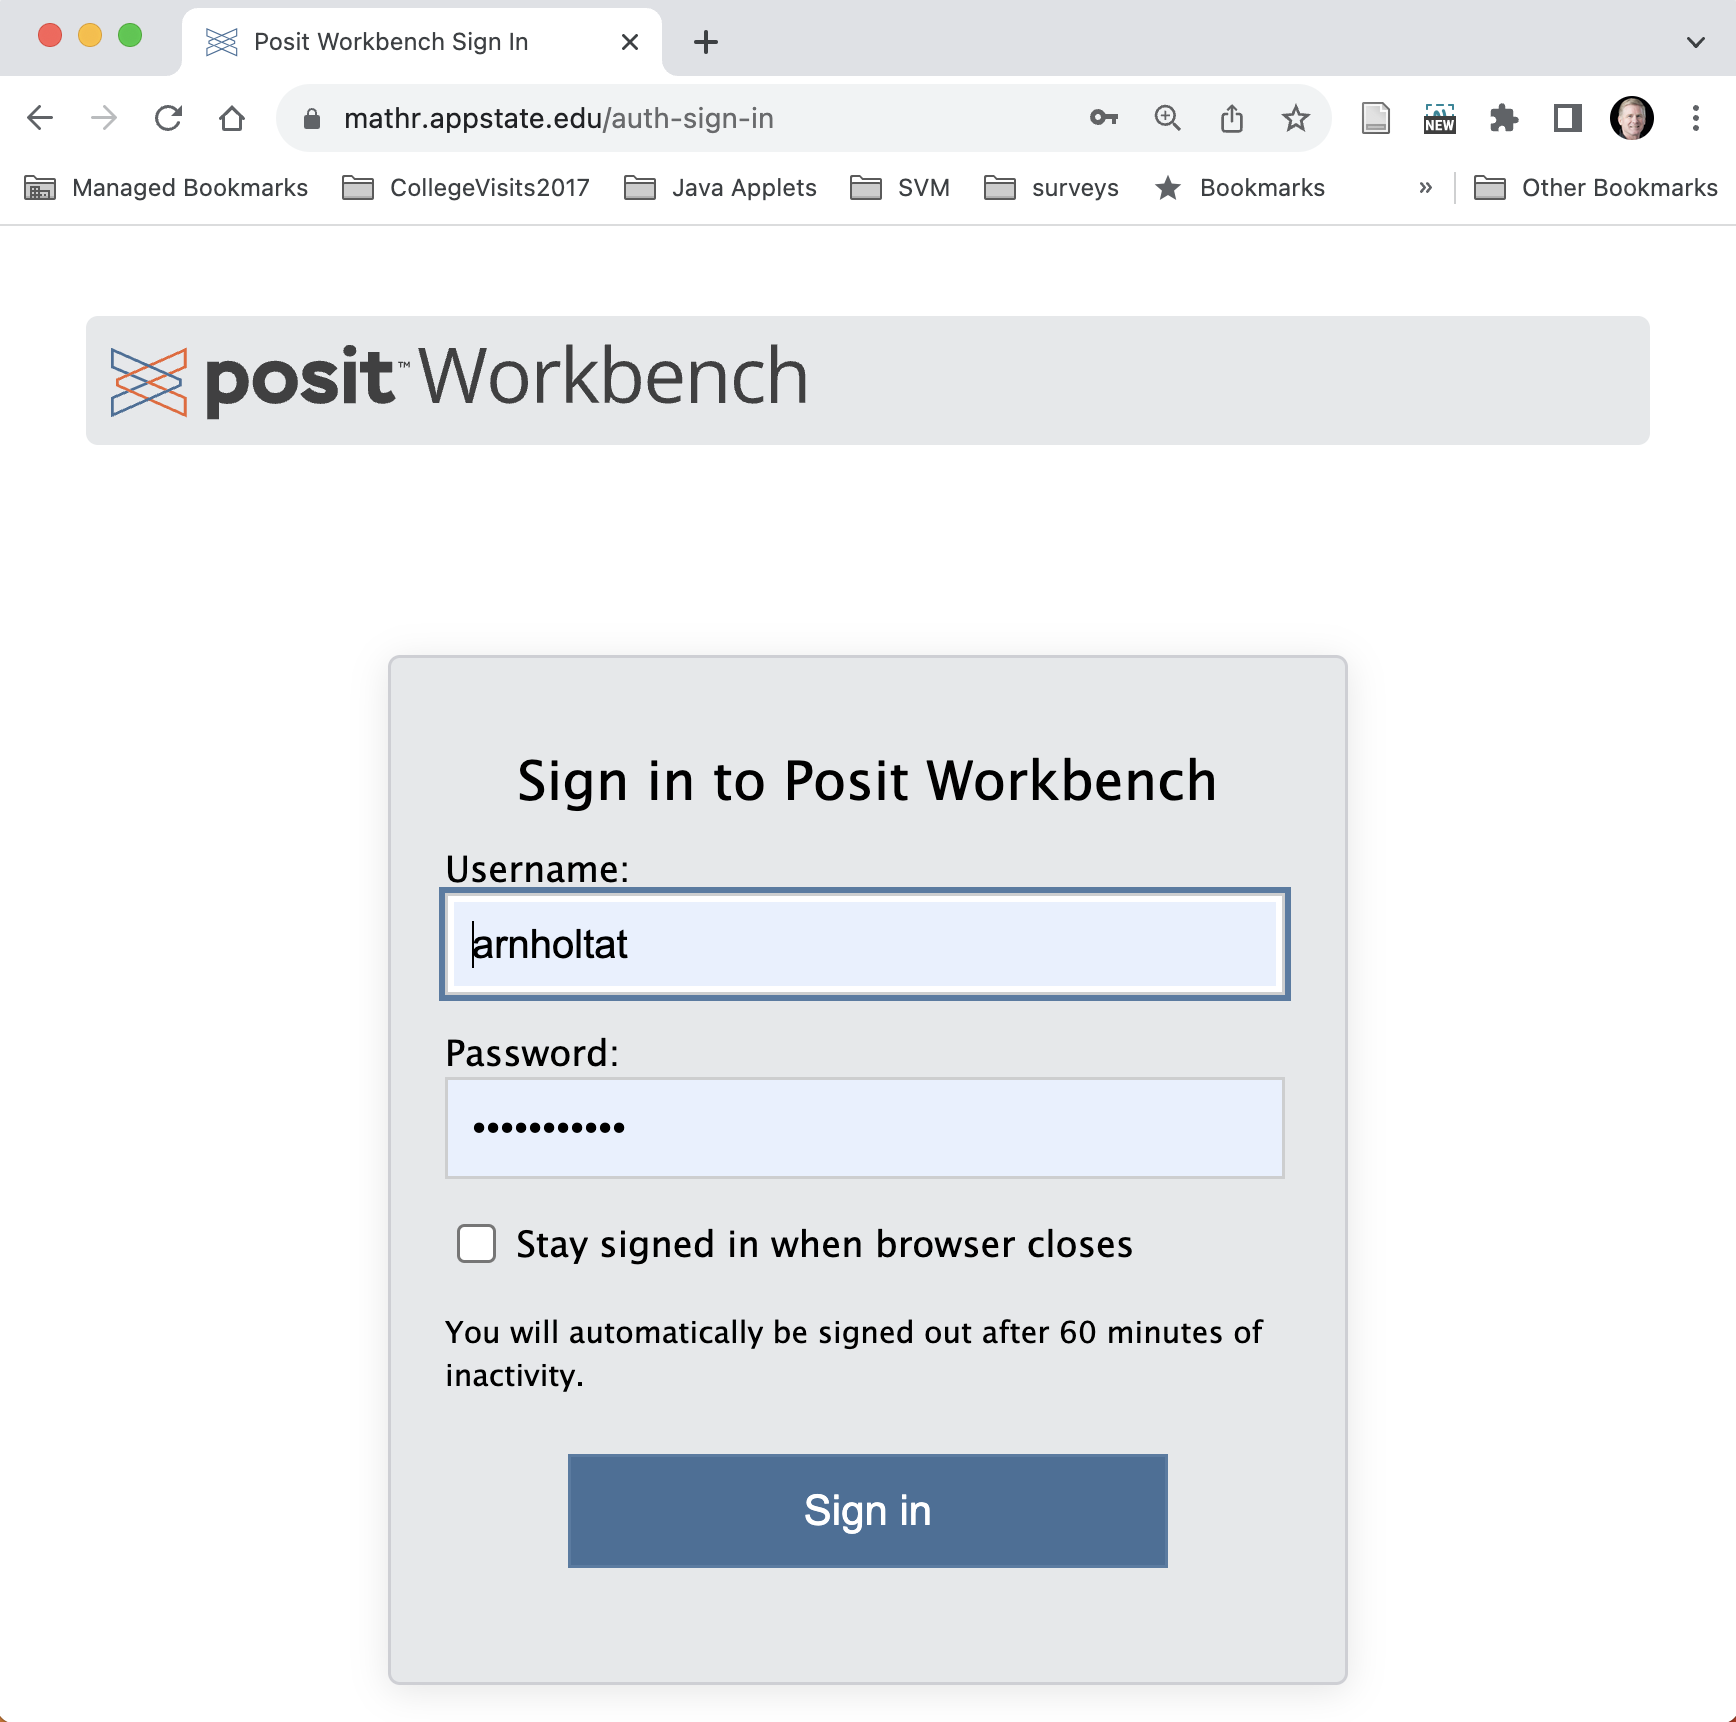
\includegraphics[width=13.56in]{POSITlogin} \end{center}

If you have problems with your Appstate Username or Password visit
\href{http://support.appstate.edu/}{IT Support Services} or call
262-6266.

\begin{center}\rule{0.5\linewidth}{0.5pt}\end{center}

\textbf{Required Technology}

\begin{itemize}
\tightlist
\item
  \href{https://mathr.appstate.edu/}{RStudio Server}
\item
  \href{https://www.datacamp.com/}{DataCamp}
\item
  \href{https://github.com/}{GitHub}
\item
  \href{https://github.com/STT3850-FALL2024}{Github Classroom
  Repository}
\end{itemize}

Note: All technology used in the class is either open source (free) or
will be accessible to students enrolled in the course for no cost.

\begin{center}\rule{0.5\linewidth}{0.5pt}\end{center}

\textbf{Assignments}

The \href{../CoursePacing/CoursePacingF2024.html}{Course Pacing Guide}
has all course assignments and due dates.

\begin{center}\rule{0.5\linewidth}{0.5pt}\end{center}

\begin{rmdnote}
\textbf{Faculty student responsibilities}

\begin{itemize}
\item
  It is my (faculty) responsibility to explain and present the material
  you need to master for this course. A detailed description of
  everything you need to do starting with day one to the Final Exam is
  provided in the course pacing guide which is available on day one of
  the course.
\item
  It is your (student) responsibility to learn the material and to seek
  help if you do not understand the material.
\end{itemize}
\end{rmdnote}

Appalachian students are expected to make intensive engagement with
courses their first priority. Practically speaking, students should
spend approximately 2-3 hours on coursework outside of class for every
hour they spend in class. For this four-hour course, you you should
anticipate 8-12 hours per week of outside work.

\begin{center}\rule{0.5\linewidth}{0.5pt}\end{center}

\textbf{How To Do Well In This Course}

The only way to learn statistics is to \textbf{DO} statistics, which
includes using statistical software. Reading the textbook, learning the
language, and practicing exercises using real data are critical to your
learning and success. Class activities and assessments have been
structured with these principles in mind.

You should read assigned textbook content and read/watch supplemental
materials prior to coming to class. When you read the assigned material,
you should complete the problems (not just read about them) on your
paper and computer. It will be easier to participate if you acquire some
familiarity with the vocabulary and methods before we start to discuss
and use them. You must ``speak the language'' (both statistics and R) to
demonstrate your knowledge effectively. If you come to class and have
difficulty following the discussion, you should make sure you have read
all of the assigned material and then go back and re-read the assigned
material a second time. Reading a technical book is not the same as a
novel. Most people, your instructor included, must read a technical
section at least twice before understanding a topic. If you are still
having challenges after reading the assigned material twice and working
the out the material on paper and the computer, it is your
responsibility to seek help. I am here to help and will be glad to
assist you in your learning process. Please make an appointment to visit
with me on my
\href{https://calendar.app.google/FS1gx8qdFUkN6Z9Y8}{calendar}.

\begin{center}\rule{0.5\linewidth}{0.5pt}\end{center}

\textbf{How To Get Unstuck}

Well constructed questions will elicit answers more rapidly than poorly
constructed questions. This
\href{https://www.youtube.com/watch?v=ZFaWxxzouCY\&list=PLjTlxb-wKvXNSDfcKPFH2gzHGyjpeCZmJ\&index=3}{video}
provides some background on asking questions. This stackoverflow thread
details how to create a
\href{http://stackoverflow.com/questions/5963269/how-to-make-a-great-r-reproducible-example/5963610\#5963610}{minimal
R reproducible example}. Please read
\href{http://www.catb.org/~esr/faqs/smart-questions.html}{How To Ask
Questions The Smart Way} by Eric Raymond and Rick Moen and heed their
advice.

\begin{center}\rule{0.5\linewidth}{0.5pt}\end{center}

\end{document}
